
A significant threat to today's computer networks are attacks that aim to gain unauthorised access to sensitive infrastructure and information, especially as the increasing rate of zero-day attacks \cite{zeroday} threatens the traditional model of signature-based network intrusion detection. Such attacks are used to gain control or access information on remote devices by exploiting vulnerabilities in network services, and are involved in many of today's data breaches \cite{mandiant2015trends}.
Anomaly-based intrusion detection methods are aimed to decrease the threat of zero-day attacks by not relying \textcolor{red}{...} on libraries of known attack signatures, but their success is currently restricted to the detection of high-volume attacks using aggregated traffic features. Recent evaluations show that the current anomaly-based network intrusion detection methods fail to detect remote access attacks reliably \cite{nisioti2018intrusion}. 

Prominent network intrusion detection methods as Kitsune \cite{mirsky2018kitsune} or DeepCorr \cite{nasr2018deepcorr} learn structures in the sizes, flags, or interarrival times (IATs) of packet sequences for decision-making. These structures reveal information about attack behaviour, but are also influenced by a number of other factors such as network congestion or the transmitted data. We define \textbf{traffic microstructures} as reoccurring patterns in the metadata of packet sequences (such as used in shallow packet inspection) within a connection, such as the packet sizes of a Diffie-Hellman exchange or typical IATs of video streaming, or patterns within the summary statistics of individual connections or short sequences observed on a host such as the pattern of port 53 (DNS) connections being followed by port 80 or 443 connection (HTTP/S). No effort has been made so far to monitor or control these factors to probe these models for specific microstructures, with the current quasi-benchmark NID-datasets pay more attention to the inclusion of specific attacks and topologies rather than the documentation of the generated traffic. 
This situation has so far led researchers to often simply evaluate a variety of ML-models on these datasets in the hope of edging out competitors, without understanding model flaws and corresponding data structures through targeted probing.
Sommer and Paxson \textcolor{red}{citation} have already \textcolor{red}{should this be in?}



%Network intrusion detection models such as DeepCorr or Kitsune \textcolor{red}{citation} increasingly rely on learning \textcolor{red}{traffic microstructures} that consist of pattern sequences in features such as interarrival time, size, or packet flags. However, there exist \textcolor{red}{little to no} research that examines common variations of benign traffic microstructures, and how attacks commonly perturb them. \textcolor{red}{Something about datasets incsufficient}. 

The aim of this thesis is to improve the understanding of traffic microstrucutres and their shaping, and to define and propose methodologies to develop machine-learning based anomaly detection methods that leverage traffic microstructures effectively.







\section{Motivation}

This section motivates the research on traffic microstructures and corresponding models and generation processes.

\subsection{The case for machine learning and anomaly-based intrusion detection}

Intrusion detection can be seen as a never ending arms-race between malicious actors on the one side that aim to access, manipulate, or damage computation infrastructure in a network, and the network operators, detection system providers and research community, on  the other. Traditionally the most common approach to network intrusion detection is based on detecting closely defined notions of attacks, known as \emph{attack signatures}. Since the late 1980's, signature based systems such as Snort or Bro \textcolor{red}{citation} have dominated the field of network intrusion detection due to high effectiveness, low false positive, and good computational efficiency. Due to their design, signature-based methods can only alert on known issues that had been categorised as threats on a signature list; zero-day attacks remain a \textcolor{red}{large vulnerability} of traditional IDSs.

In the 1990's, anomaly-detection emerged as a complementary detection tool by training machine learning or statistical analysis on large traffic datasets in order to detect variants on existing attacks or entirely new classes of attacks. However, inconsistent detection results and high false positive rates lead many administrators to believe machine-learning based intrusion detection to be unreliable, computationally too expensive, and headed for a slow death.
In 2010, Sommer and Paxson discuss a number of reasons why machine-learning based detection methods failed to provide similar levels of success as their signature-based counterpart.

However, ...

Machine-learning and anomaly-based intrusion detection solutions are finding more widespread industrial application in products from companies such as Crowdstrike, Darktrace, \textcolor{red}{citation}. Furthermore, the rise of cloud computing has shifted the computational burden of complex intrusion detection systems from the monitored hosts to the cloud.

\textcolor{red}{Current detection methods are predominantly based on the analysis of previously identified attack signatures, which provides great reliability and low false alert rates. However, these methods are dependent on an updated attack signature database and provide no protection against previously unseen attacks. With attackers having access to more resources than ever, custom-built malware is becoming more common to circumvent signature-based detection. 
Another approach that has recently gained traction in commercial deployment is based on detecting malware and other undesired activity as anomalous behaviour when compared to benign computer activity. In this approach, known as \textbf{network anomaly detection} after Denning \cite{denning1987intrusion}, models must quantify the behaviour of normal network behaviour to be independent of a narrowly defined notion of malicious activity.
}


\subsubsection{SPI and microstructures}

Many ISP solutions rely on \emph{deep packet inspection} (DPI), where payloads of packets are scanned for attack signatures or anomalies. While this offers a direct view at the content of communications, it raises several problems: The computational overhead of DPI is large and scales directly with the amount of transferred data. Furthermore, DPI infringes user privacy when scanning the content of messages, potentially allowing the operator to access the vast amount of personal information sent over the internet. Finally, DPI is incapable of processing encrypted traffic, an issue that malicious actors increasingly exploit. \textcolor{red}{Some IDS-providers have started to decrypt any transferred traffic in a man-in-the-middle manner, but the ethical legitimacy of such approaches are at the very least controversial.}

\emph{Shallow packet inspection} (SPI) in contrast only inspects packet headers and is therefore computationally less expensive as well as robust against encryption and to some degree application evolution \textcolor{red}{citation}. SPI is used both by rule- and signature-based systems such as Snort, as well as by an ever increasing number of machine-learning based methods that attempt to make broad generalities about traffic solely from evaluating packet headers. \textcolor{red}{insert some statistic how many}.

For this, many traffic classification and anomaly-detection approaches leverage small-scale structures visible in the sizes, interarrival times, flags, port, etc. of packet sequences, which we call \emph{traffic microstructures}. \textcolor{red}{insert image and example here}. 

However, there exists no systematic description of these structures, and their usage is mostly only justified from high-level argumentation without any examination about the influences on them or their prevalence in the respective datasets used for evaluation. \textcolor{red}{some additional arguments about model development?}


\subsection{Lack of model development in NID}


\subsection{Dataset problems and lack of labels}




Newer models clearly leverage microstructures

However, traffic opaque 

...

\section{Contributions}

This thesis provides extensive examinations of the necessary requirements on traffic generation and traffic microstructures to enable the effective training and improvement of anomaly detection models. The here presented findings provide \textcolor{red}{...}

More specifically, we examine how current machine-learning based SPI-detection methods are designed and their requirements on comprehensive and realistic datasets to generate models that generalise well on persistent traffic microstructures. We establish our findings with several experiments and empirical evidence of shortcomings from existing datasets\textcolor{red}{...}.

\begin{figure}
\centering
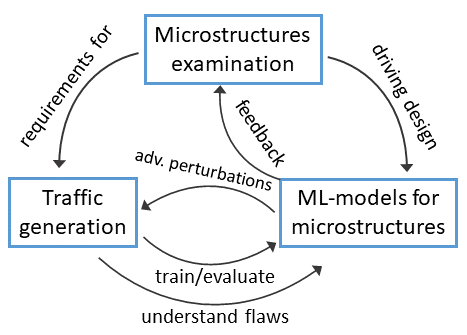
\includegraphics[width=0.6\textwidth]{images_introduction/Themes.PNG}
\caption{Three main themes of this thesis.}\label{Fig:themes}
\end{figure}

This thesis then proposes DetGen, a traffic generation paradigm to provide control over various influence factors that shape traffic microstructures. The goal of DetGen is to provide researchers with extensive ground truth information and enable the generation of customisable, scalable, and controllable datasets with realistic levels of microstructure diversity. We examine with the level of control DetGen provides with a number of experiments to compare with existing traffic generation techniques. 

We demonstrate the benefit of precise traffic control and corresponding ground truth labels by probing two state-of-the-art (SOTA) NID models to understand where they fail and how they can be improved. We identify design flaws with regards to specific microstructures, and can correspondingly improve the detection performance by several percentage points. These examinations also serve as examples how the model development process in NID can be \textcolor{red}{extended} to improve existing models and build up on previous results.

Building up from these results, we propose CBAM, an anomaly detection model that detects low-volume access attacks as deviations from \textcolor{red}{persistent} flow microstructures. CBAM is trained as a self-supervised traffic language model and outperforms current state-of-the-art methods by \textcolor{red}{xxx points}. We examine persistent microstructures that are perturbed by specific attacks, and how CBAM detects these perturbations. The output of CBAM also provides valuable insights into the frequency, clustering, and evolution of microstructures in real-world traffic.

Lastly, we examine how attackers can perturb traffic in a stepping-stone attack in an adversarial way to prevent models from identifying the corresponding microstructures. We use DetGen to generate controllable stepping-stone attack data to identify which level of perturbations are required to prevent detection. We then evaluate several models with different detection methodologies on this data and conclude that realistic adversarial perturbations can evade all current methods.

\subsection{Thesis overview}

\paragraph*{Chapter 2} provides the reader with background information on network traffic and attacks, machine-learning based network intrusion detection and explains the necessary concepts of machine-learning based anomaly detection for sequential data streams. The chapter highlights important NID models that leverage traffic microstructures, and discusses existing datasets and synthetic traffic generation as well as their current shortcomings, as well as related studies on traffic structures.

\paragraph*{Chapter 3} introduces DetGen, a framework that provides small-scale traffic generation specifically aimed for machine-learning based intrusion detection. The chapter starts with the identification of four major shortcomings of existing NID-datasets regarding the training of machine-learning models that leverage traffic microstructures. The chapter then defines four requirements that a machine-learning-focused traffic generation framework must fulfil. The chapter then provides results from several experiments to demonstrate the lack of model \textcolor{red}{generalisability} when trained on data not meeting these requirements. 

\begin{figure}[t]
\centering
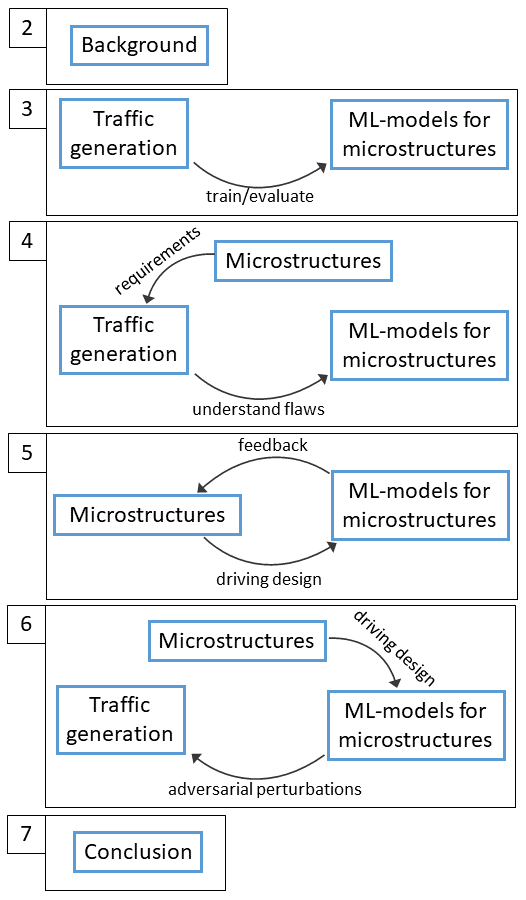
\includegraphics[width=0.6\textwidth]{images_introduction/Thesis_structure.PNG}
\caption{Chapter structure of this thesis.}\label{Fig:structure}
\end{figure}

\paragraph*{Chapter 4} builds up on the results in Chapter 2 by experimentally examining the influence of several factors on traffic microstructures and the level of control that DetGen provides. The chapter then provides two case-studies on how to produce traffic effectively to probe a state-of-the-art traffic classifier, and why a certain degree of generative determinism is required for this to isolate the influence of traffic microstructures. 

\paragraph*{Chapter 5} introduces CBAM, an anomaly detection model that detects low-volume access attacks as deviations from \textcolor{red}{persistent} flow microstructures. The chapter explains the reasoning for CBAM's design in order to learn specific microstructures in a self-supervised manner, and how attacks perturb these microstructures. The chapter then provides detection results and a comparison to three benchmark (SOTA) models, before examining long-term stability of the learned structures and current shortcomings on real-world datasets.

\paragraph*{Chapter 6} explains the procedure of a stepping-stone attack, common techniques based on SPI to detect them, and how attackers introduce perturbations to evade detection. The chapter then provides  results from data with varying degrees of introduced perturbations and the corresponding performance results of seven stepping-stone detection methods.

\paragraph*{Chapter 7} concludes this thesis, provides a crictical perspective on the presented results, and gives an outlook to future work in this area.